\documentclass[a4paper, 12pt]{article}

%\usepackage{cmap}
\usepackage[T2A]{fontenc}
\usepackage[utf8]{inputenc}
\usepackage[english, russian]{babel}
\usepackage{graphicx}
\usepackage[top=1in, bottom=1in, left=3.2cm, right=2.6cm]{geometry}
\graphicspath{./}
\usepackage{biblatex}
\addbibresource{lib.bib}
\linespread{1.5}

\usepackage{listings}
\usepackage{color}
\usepackage{amsmath}

\begin{document}
	
\begin{titlepage}
	\fontsize{12pt}{12pt}\selectfont
	\begin{figure}[t!]
		\centering
		
\includegraphics[scale=0.8]{bmstu}
	\end{figure}
	
	\noindent\rule{15cm}{3pt}
	\newline\newline
	\noindent 
	ФАКУЛЬТЕТ 
	\underline{«Информатика и системы управления»} \newline\newline
	
	\noindent КАФЕДРА \underline{«Программное обеспечение ЭВМ и информационные технологии»}\newline\newline\newline\newline\newline\newline
	
	\centering {\LARGE Отчет по рубежному контролю № 1}
	\vspace{3mm}
	
	\centering {\LARGE По курсу "Анализ Алгоритмов"
		\vspace{10mm}	
		
		\centering \bf Сравнение алгоритмов полного перепора и бинарного поиска в массиве}
	\vspace{10mm}
	
	
	\begin{flushright}
		{\large	Студент:\\ Турсунов Жасурбек Рустамович \\ Группа: ИУ7-56Б
			\vspace{5mm}
			\\Преподователи: \\ Волкова Лилия Леонидовна \\ Строганов Юрий Владимирович}
	\end{flushright}
	
	\begin{center}
		\vfill
		Москва, \the\year
		~г.
	\end{center}
\end{titlepage}

\tableofcontents
\clearpage
\newpage


\section{Постановка задачи}
\hspace*{5mm} Изучить алгоритмы полного перебора и бинарного поиска элемента в массиве. Провести анализ на полученных данных и определить самый быстрый алгоритм. Размер массива будет варьироваться от 1000 до 10000.
Для алгоритма бинарного поиска необходимо подготовить данные, а именно отсортировать их заранее. Для сортировки будет использована внутренная функция Python - sort(). Замер времени будет произведен функцией из библиотеки time - perf-counter. 
	

\section{Решение}
	\hspace*{5mm} \textbf{Алгоритм полного перебора} не обладает специфичными действия. Этот алгоритм поэлементно проходится по элементам массива до тех пор, пока не найдет нужный элемент. В случае пустого массива или поиска несуществующего элемента, алгоритм вернет значение None.
	\\\hspace*{5mm} \textbf{Алгоритм двоичного поиска} применяется к заранее упорядоченному словарю. Процесс двоичного поиска можно описать при помощи шагов:
	\begin{enumerate}
		\item получить значение по индексу, находящееся в середине массива, и сравнить его с данным;
		\item в случае, если значение меньше (в контексте типа данных) данного, продолжить поиск в левой части словаря, в обратном случае – в правой;
		\item на новом интервале получить значение по индексу из середины этого интервала и сравнить его с данным;
		\item продолжать поиск до тех пор, пока найденное значение по индексу не будет равно данному.
	\end{enumerate}
	\hspace*{5mm}Поиск в массиве с использованием данного алгоритма в худшем случае будет иметь трудоемкость $O(log_2N)$, что быстрее поиска при помощи алгоритма полного перебора. Но стоит учитывать тот факт, что данный
	алгоритм работает только для заранее упорядоченного массива. В случае большого объема данных и обратного порядка сортировки может произойти так, что алгоритм полного перебора будет эффективнее по времени, чем
	алгоритм двоичного поиска. 
	
 


\section{Листинг кода}

	На листингах 1, 2 представлена реализация алгоритмов поиска в словаре.
	\definecolor{codegreen}{rgb}{0,0.6,0}
	\definecolor{codegray}{rgb}{0.5,0.5,0.5}
	\definecolor{codepurple}{rgb}{0.58,0,0.82}
	\definecolor{backcolour}{rgb}{0.95,0.95,0.92}

	\lstdefinestyle{mystyle}{
		backgroundcolor=\color{backcolour},   
		commentstyle=\color{codegreen},
		keywordstyle=\color{magenta},
		numberstyle=\tiny\color{codegray},
		stringstyle=\color{codepurple},
		basicstyle=\ttfamily\footnotesize,
		breakatwhitespace=false,         
		breaklines=false,                 
		captionpos=b,                    
		keepspaces=true,                 
		numbers=left,                    
		numbersep=5pt,                  
		showspaces=false,                
		showstringspaces=false,
		showtabs=false,                  
		tabsize=4
	}

	\lstset{style=mystyle}

	\begin{lstlisting}[language=Python, caption = Алгоритм полного перебора]
def full_iteration(data, val):
	if len(emails) == 0:
		return None
	for i in range(len(data)):
		if data[i] == val:
			return i+1
	return None
	\end{lstlisting}
\begin{lstlisting}[language=Python, caption = Алгоритм бинарного поиска]
def bin_search(data, val):
	result = None
	if len(data) == 0:
		return result
	mid, low, high = len(data) // 2, 0, len(data) - 1
	while data[mid] != val and low <= high:
		if val > data[mid]:
			low = mid + 1
		else:
			high = mid - 1
		mid = (low + high) // 2
	if low < high:
		result = mid 
	return result
\end{lstlisting}

\section{Тестирование функций}
	\hspace*{5mm} На рисунке 1 приведены результаты функциональных тестов для функций, реализующих алгоритмы поиска в массиве.
	\clearpage
	\newpage
	\begin{figure}[h]
		\centering 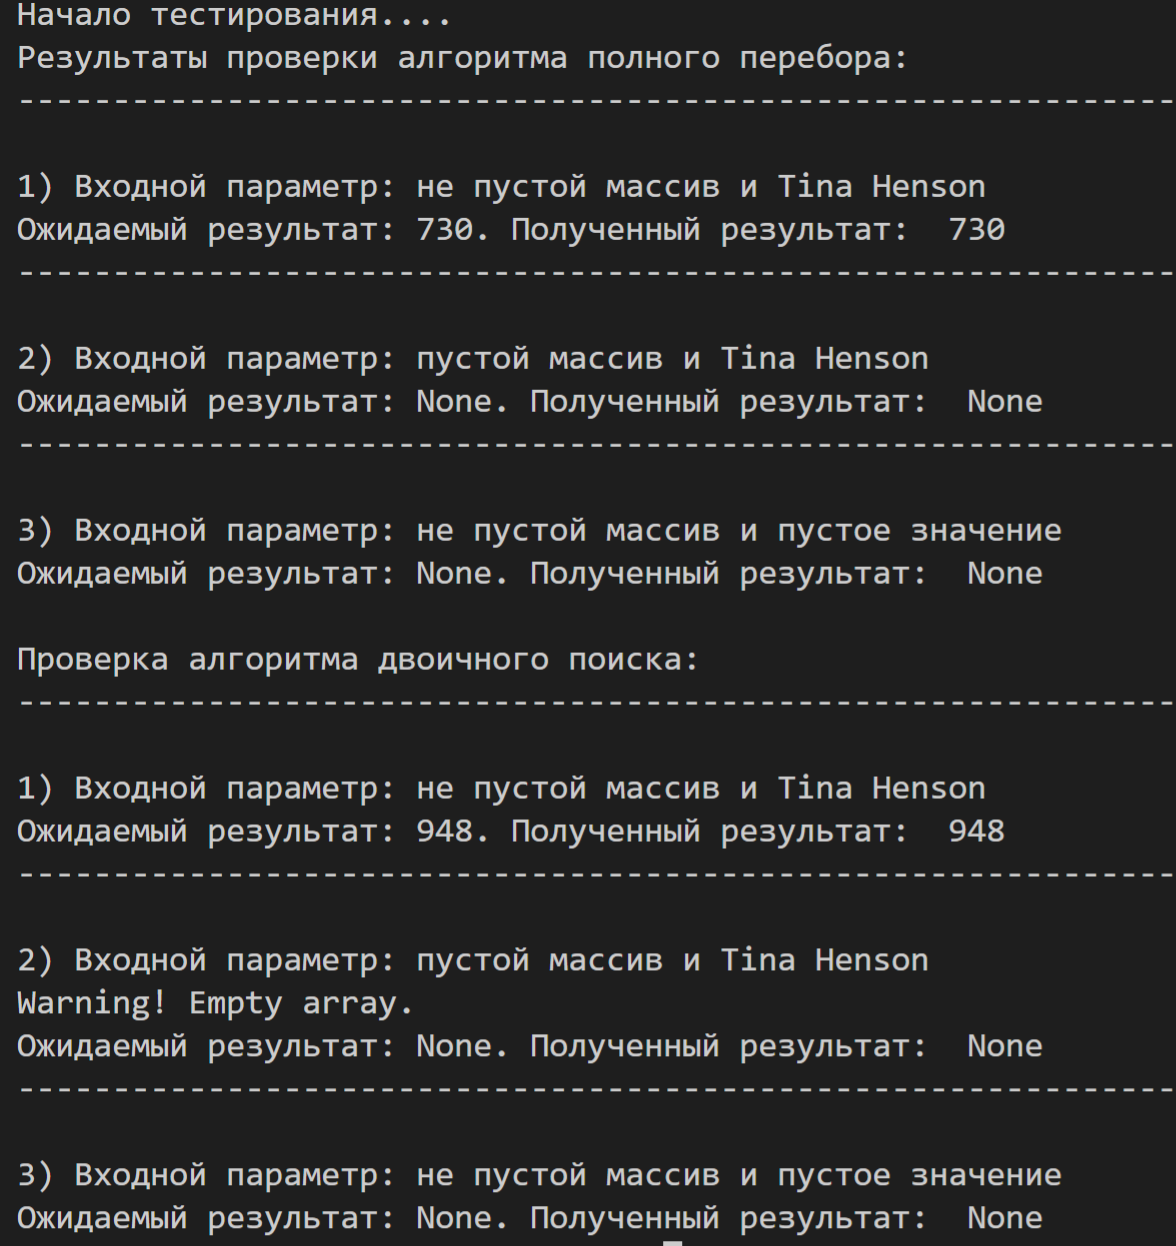
\includegraphics[scale=0.9]{tests}
		\centering\caption{Результаты функциональных тестов.}
	\end{figure}
	Все тесты прошли успешно.	 	


\section{Примеры работы}

	\hspace*{5mm} На рисунке 2 показан пример работы программы. На вход подается массив значений и значение которого требуется найти. На выходе получаем индекс элемента. 
	\clearpage
	\newpage
	\begin{figure}[h]
		\centering 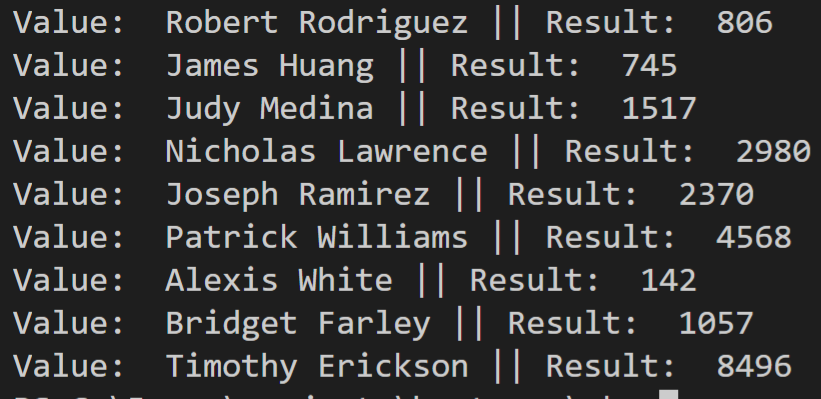
\includegraphics[scale=1.4]{res}
		\centering\caption{Пример работы программы.}
	\end{figure}

\section{Анализ полученных данных}
\hspace*{5mm} На рисунке 3 показаны результаы замера времени для алгоритма полного перебора и бинарного поиска.
\begin{figure}[h]
	\centering 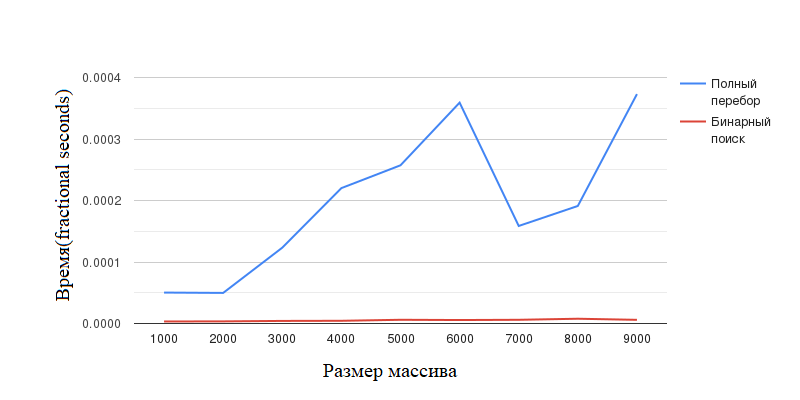
\includegraphics[scale=1.7]{chart}
	\centering\caption{Результаты проведенного анализа.}
\end{figure}
\\ \hspace*{5mm} Из полученного графика можно сделать вывод, о том что бинарный поиск в разы быстрее алгоритма полного перебора. При замере времени для бинарного поиска, не учитывалось время сортировки, которое может быть довольно длительным. 

\section*{Вывод}
\addcontentsline{toc}{section}{Вывод}
\hspace*{5mm} В ходе работы был реализован алгоритм полного перебора и бинарного поиска в массиве. Также проведен анализ замера времени этих алгоритмов.

\end{document}